\documentclass[fleqn,10pt]{wlscirep}
\usepackage[utf8]{inputenc}
\usepackage[T1]{fontenc}
\usepackage[english]{babel}
\usepackage{siunitx}
% Additional packages (Jero)
\usepackage{listings} % For inline code
\usepackage{subcaption} % For subfigure commands


% ==== TO DO NOTES BLOCK ====
% Defining some custom colors cause importing the xcolor package with todonotes raises issues
\definecolor{MyPlum}{RGB}{142, 69, 133}
\definecolor{MyOliveGreen}{RGB}{107, 142, 35}
% Importing xargs to use more than one optional parameter in new commands
\usepackage{xargs}
% Importing todonotes
\usepackage[colorinlistoftodos, prependcaption, textsize=tiny, textwidth=1.5cm,color=red!20]{todonotes}
% Defining new commands for faster formatting (two formats for my notes and one for Lucas')
\newcommandx{\todoj}[2][1=]{\todo[author=Jero,linecolor=MyOliveGreen,backgroundcolor=MyOliveGreen!25,bordercolor=MyOliveGreen,#1]{#2}}
\newcommandx{\todof}[2][1=]{\todo[author=Jero,linecolor=MyPlum,backgroundcolor=MyPlum!25,bordercolor=MyPlum,#1]{#2}}
\newcommandx{\todol}[2][1=]{\todo[author=Lucas,linecolor=blue,backgroundcolor=blue!25,bordercolor=blue,#1]{#2}}
\newcommandx{\repl}[2][1=]{\todo[noline,backgroundcolor=blue!22,bordercolor=blue,#1]{#2}}
% Format:
% \todo[author=YourName,color=blue!20]{Customized to-do note.}
% List of to-do notes: \listoftodos
% For more options, the docs are actually pretty good: https://ctan.org/pkg/todonotes
% ===========================


\title{Assessing the Cancer Stem Cell distribution in tumorspheres using data science tools.  }

\author[1]{Jer\'onimo Fotin\'os}
\author[2]{Mar\'ia Paula Marks}
\author[1,*,+]{Lucas Barberis}
\author[2,+]{Luciano Vell\'on}
\affil[1]{IFEG, FAMAF, CONICET, UNC, C\'ordoba, Argentina}
\affil[2]{Stem Cells Lab, IBYME, CONICET, Buenos Aires, Argentina}

\affil[*]{lbarberis@unc.edu.ar}

\affil[+]{these authors contributed equally to this work}

\keywords{imaging processing, tumorsphere assay, cancer stem cells}

\begin{abstract}
In previous theoretical research, we inferred that Cancer Stem Cells (CSCs), the cells that presumably drive tumor growth and resistance to conventional cancer treatments, are not uniformly distributed in the bulk of a tumorsphere. This knowledge is useful for mathematical modeling, which most of the time assumes uniformity as a simplification. The CSCs distribution in a 3D tumor model, such as a tumorsphere, is crucial not only for understanding and designing novel and more specific anti-CSC therapies but, also for the design and check of mathematical and computational models.  

In this article, we present a method to process confocal images from tumorsphere assays and measure the amount and location of their Cancer Stem Cells. Guided by a previous computational model, we conclude that the distribution of Cancer Stem Cells in an experimental tumorsphere must be non-homogeneous.

\end{abstract}
\begin{document}

\flushbottom
\maketitle

\thispagestyle{empty}


\section{Introduction} \label{s: intro}
% define CSC, son poco accesibles y como se las consigue
Cancer Stem Cells (CSCs) are defined by their capacity to replicate making copies of themselves or to differentiate giving rise to phenotypically diverse cells. They are resistant to conventional anti-cancer treatment, being thus implicated in disease recurrence and metastasis\cite{Al-Hajj, Kakarala}. One of the main barriers to the development of CSCs-targeted therapies is their scarcity in vivo, limiting their availability as experimental systems for pharmaceutical development, and raising the need for production at a scale large enough to fulfill academic and industry requirements. A common solution is the anchorage-independent growth of cancer cells to generate a 3D culture of epithelial cells\cite{Dontu} enriched in cells with CSCs-like properties, \todol{la frase que sigue no entiendo por que' es importante. Como esencial no lo es, sencillamente describe el ensayo de esferas como un ensayo de resistencia a anoikis, es decir, a la muerte por falta de adhesión a un sustrato. (J) A mí me gusta esta aclaración, quizás pondría una coma antes de enriched y sacaría el punto antes de since.} since most epithelial cells are killed by anoikis\cite{Ehmsen}. Thus, taking into account the limitations of this assay\todol{No s\'e a que limitaci\'on s\'e refiere. Las limitaciones son: cuidar la densidad de cultivo ya que las esferas deben ser clonales y que no detecta células madre quiescentes ya que quedarían como célula única al no dividirse, están enumeradas en la referencia, pero si es conflictivo saco esa parte. (J) Quizás convenga mencionarlas brevemente o poner la referencia al lado de limitations. (L) no, corta demasiado la frase, está bien así porque la referencia afecta a toda la frase}, the resulting tumorspheres are formed by the clonal expansion of a single cell, instead of the self-aggregation of existing cells\cite{Pastrana}.

%es dificil e ineficiente hay que hacer algo mejor
Still, routinely used cell culture techniques are material- and labor-consuming tasks that generate a great amount of inter-culture variability and contamination risks. Moreover, traditional cell culture at a large scale is also cost-ineffective in terms of the high investment in cell culture media and growth factors. 
In this context, developing forefront, high-throughput screening platforms to identify cytotoxic inhibitors and/or differentiation-promoting agents targeting CSCs becomes of paramount importance. This would require the optimization of a series of bioprocesses that enable the massive culture of undifferentiated cancer cells and the analysis of high volumes of data. 

% hay que saber donde est'a en el cultivo y se usa sofware y matem'atica
One critical downstream part of such bioprocesses is to assess the cellular response in terms of viability and/or stemness markers, which requires external software for image analysis and segmentation to quantify the relative differences among treatment groups. Even though high-throughput cytometric methods have been developed\cite{Kessel}, there is still the need to know the exact identification, location, and targeting of putative CSCs. This would help the modeling of CSCs dynamics, allowing the development of cost-effective and predictive tools for the examination of tumor evolution and response to therapy.
%
Mathematics, physics, and computational modeling offered positive prospects in cancer research,\todoj{Sounds a bit unnatural.} being widely used. Many biological problems, including cancer disease, demand methods and techniques requiring applied mathematics, statistics, fluid and phase transitions physics, population dynamics, and computation\cite{laporta, bull2022hallmarks, Vieira}. Indeed, analytical mathematical methods allowed us to estimate the expected fraction of CSCs for tumorspheres in different culture conditions\cite{benitez2019, barberis2021diff, benitez2021} and the effect of specific therapies on their development\cite{fotinos23} among other theoretical results\cite{Condat2006, Delsanto2008, Menchon2011, Barberis2015}.  

%modelo computacional previo TIENE que decir que son los PATHS y como se forman
We have also computationally simulated the growth of a colony of cells in two dimensions using an Agent-Based Model (ABM) that mimics basic features of CSCs proliferation to form a spheroid\cite{barberis2021percolation}. The simulated spheroid grows from a single CSC and the cells can undergo mitosis at a fixed rate (the population doubling time or PDT). Depending on the intrinsic and extrinsic (micro-environment) signals, the CSC will replicate generating another CSC with a certain probability $p_s$, \todoj{I'd say smth like 'yielding a DCC otherwise'.}or it will differentiate generating a \emph{differentiated cancer cell} (DCC). This simplified model allowed us to estimate the total number of CSCs, the fraction of CSCs situated on the periphery of the colony, and the size of the whole spheroid, showing that these traits are dependent on  the replication probability ($p_s$) of the CSC. Indeed, simulating with intermediate replication probabilities, we observed active CSCs at the border of the colony and detected that they form a path that links the center of the colony with its border. Furthermore, an increase in the replication probability led, as expected, to a large CSCs population that overtook the system. This last situation may describe most experimental conditions used for culturing tumorspheres \cite{chen2016,wang2016, Dontu, Leis, Marks2024} and agrees with our previous mathematical models \cite{benitez2019, barberis2021diff, benitez2021}.

%deteccion de CSC con Data science
Inspired by these simulations, we generated tumorspheres from MCF-7 cells and analyzed them by confocal microscopy.  We developed an advanced computational method to detect the expression and distribution of the stem-like cells (Sox2-positive cells), under the assumption\cite{Leis} \todoj{Sox2 (lower case?) shouldn't be in parentheses if it's going to be refered to outside them.} that this stemness factor is expressed in tumorspheres from cell lines and primary cultures. The processed images were used to study the distribution patterns of CSCs employing statistical tools that validate our main computational finding: that CSCs are heterogeneously distributed in a tumorsphere. 

Summarizing, we measured a non-homogeneous distribution of CSCs in tumorspheres after a computational model predicted it. In particular, we report a protocol to analyze confocal images of tumorspheres that were stained with a stemness marker, to statistically infer the more suitable threshold to determine which cells in the culture belong to the stem phenotype. We highlight the capability of our method to extract data from the experiments allowing direct comparison with simulated cultures. With this purpose, theoretical work was useful to drive experiments and, conversely, ad hoc experiments become crucial to develop more accurate theoretical work.      


\section*{Results and discussion} \label{s: results}
%intro
According to simulations\cite{barberis2021percolation}, CSCs must be connected in tumorspheres forming ``paths'' that join the center of the spheroid with its border. To assess this, we performed tumorspheres assays where MCF-7 cells in suspension culture\todoj{suspension cultures?} proliferate in a solution enriched in growth factors to ensure a large fraction of CSCs. After 9 days of growth, we collected the spheroids and attached them to a slide by cytocentrifugation. Due to the centripetal \todo{no ser\'ia centr\'ifuga?}forces, their spheroidal shape may be lost, becoming discs smashed against the slide, however, the structure of the tumorsphere is maintained. We stained the slides to detect the location of all cellular nuclei (DAPI) and the corresponding primary and secondary antibodies needed to detect the position of the stem cells (SOX2). Finally, we took pictures using a confocal microscope, slicing\todoj{this makes me think that we physically slice the spheroid} the spheroids and obtaining a full 3D reconstruction. Because of the smashing of the spheroids, only one or two slices of the imaging \todo{image?} were needed to observe all the cells present in them. These images were processed with a Data Science approach, using computer vision and statistical analysis techniques, among others. The result of the process allows us to mathematically reconstruct the discs, specifying the position of all their cells, marking those that are candidates to be CSCs and statistically deciding which ones are in fact CSCs.
The experiment and the image processing procedure are fully detailed in the \ref{s: methods} Methods section.

%For each layer, we used three optical channels: the ground channel is a complete view of the spheroids, and the other two correspond to DAPI and SOX2 fluorescence channels belonging to the mark of the nuclei and the stem cells respectively.  


\subsection*{The Cancer Stem Cells distribution. }

Our main results are summarized in Fig. \ref{fig: blue red}\todof{We need to redo this merged image preserving quality. Also, the caption needs a bit more explanation of the selected slices: which is on top of which, and the fact that those slices allowed to reconstruct the entire corresponding spheroid.}, in which we can observe the distribution of the two cell phenotypes:  CSCs in red and DCCs in blue. We present three representative examples belonging to the reconstruction of three different spheroids. After the filtering and reconstruction process of the confocal images, we obtained pictures of the cell's distribution as a Voronoi tessellation (see Methods section). That is, each cell is represented, in Fig. \ref{fig: blue red}, as a polygon whose centroid coincides with the centroid of the corresponding cell in the pictures. Note that this representation is just an approximation of the shape of the cell that allowed us to quantify the SOX2 content inside the cell and decide, using statistical tools, if the cell belonged \todoj{Maybe 'if the cell expressed a stem of differentiated phenotype'; I don't like \textit{belong} in there.} to the stem or to the differentiated phenotype. After the whole process, the CSCs become represented by red polygons and the DCCs by blue polygons. 
\todo[inline, author=Jero]{I think we should replace \textit{spots} by \textit{stains}. Spot means place; stain transmits the intended idea.}

\subsubsection*{Spots in the border}

Our first example, labeled {\textsf Sph4, slice2} as in raw data files, a spheroid that has not grown much is depicted in Fig. \ref{fig: blue red}A. Considering the different proliferative capacity of the cells in these culture conditions and the possibility of differential access to the growth factors, we expect inter-spheroid variability in both the number of cells and the CSCs fraction. In this case, the spheroid had less than a hundred cells, with half of them being CSCs, cf. \todoj{Note: the abreviation of \textit{confer} is either \textit{cf.} or \textit{cfr.}, not 'c.f.'.} Table \ref{tab: experimental values}. \todof{In Table 1's caption, I'd replace \textit{the path hypothesis} for \textit{simulations}, or I'd explain what we mean by it.} There is an evident higher concentration of the CSC in the core of the spheroids, which could be explained by the model used in our simulations: the first CSC has a given chance of generating another CSC but, when one of these CSCs differentiates the first time, its lineage will only contain DCCs that will surround its stem mother. The only exception is when a DCC cannot undergo mitosis in a nearby place, already occupied by a CSC. Indeed, this CSC will continue generating other CSCs until one of them becomes differentiated, leaving in the process a path of CSC among DCCs. This is exactly what is shown in panel (A) of Fig. \ref{fig: blue red}: at an early stage, red CSCs become surrounded by blue DCCs in the lower portion of the spheroid. However, three CSCs were able to initiate paths that extend to the periphery of the spheroid. The result is that CSC will form spots in the border of the spheroid.


A larger growth rate is associated with the case labeled {\textsf Sph3, slice 3} shown in Fig. \ref{fig: blue red} (B), where the spheroid has more cells than the one shown in panel (A). Its CSC fraction is 64\%, larger than the 54\% of the previous case, a result almost trivial that supports \todof{I don't see how one thing implies the other, but more importantly, that is not a \textbf{current} modeling hypothesis, but a former one.} our strongest modeling hypotheses: the growing rate can only be measured for the bulk of the cells, thus, the outcome of the mitosis of a CSC is given just by a probability rather than a specific growth rate for each cell phenotype\cite{benitez2021}. \todoj{Connector missing. Perhaps something like: \\ Moreover, \textit{while} the quantitative... (must change), the qualitative... (remains the same).} However, the quantitative results reported in Barberis, 2021\cite{barberis2021percolation} must be significantly different when we shift from two to three dimensions, the qualitative ones remain the same: the CSCs will form paths and be heterogeneously distributed, forming ``stains'' at the border (surface) of the spheroids after approximately one week.  

In this example, we can also appreciate the deformation produced by the smashing against the slide. Some DCCs appear in the bulk of the disk surrounded by CSCs. These DCCs \todof{Or they were just surrounded by CSCs, depriving them of space to reproduce. We don't want to give the impression that the model can't deal with DCCs near the center of the spheroid.} initially belonged to the border of the spheroid and reached the center after centrifugation. In this way, it is easy to understand why cells closer to the center of the disk could be a mix of original center cells and some of the periphery. However, there is no way in which cells at the border of the spheroid could originally be from near the spheroid center.




\begin{figure}[h!]
    %%
    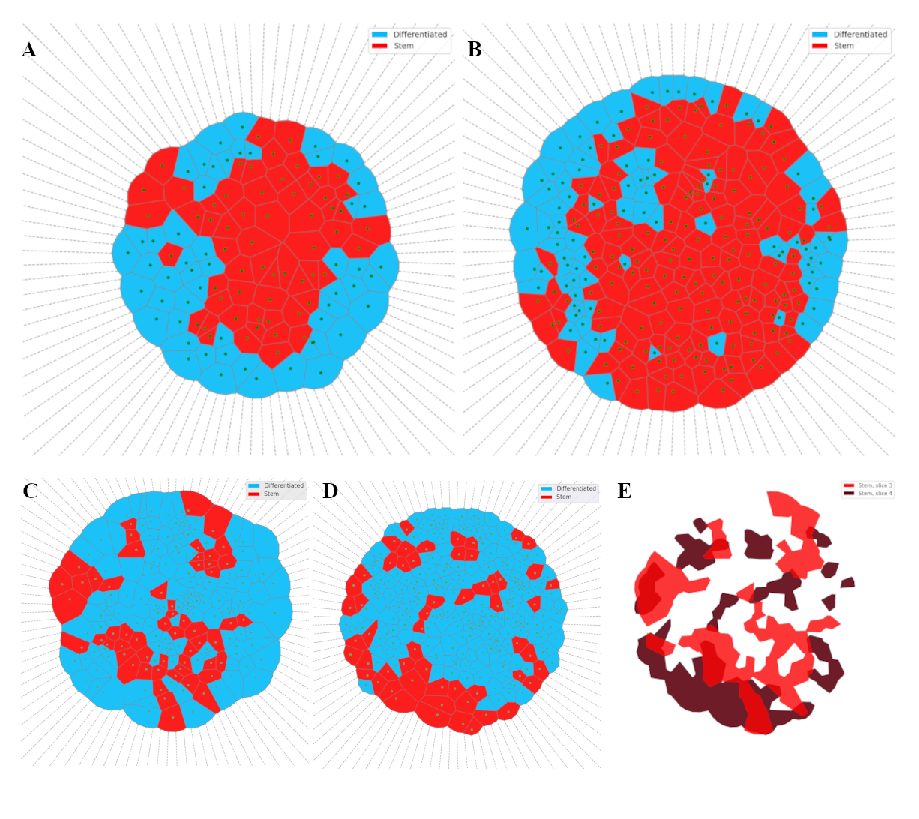
\includegraphics[width=\linewidth]{images/voronoi.eps}
    %%
    \caption{\emph{Final reconstruction of the spheroids' slices (image processing end result).} For different slices (i.e., focal planes) of the experimental spheroids, cells are shown approximated by polygons. The polygons representing CSCs are colored in red, and the ones representing DCCs, in blue. It is evident (but proven later) that the CSCs are not uniformly distributed in any image, and form stains at the border of the aggregate. The panels correspond to: \textbf{A} {\textsf Sph4, slice 2}; \textbf{B} {\textsf Sph3, slice 3}; \textbf{C} {\textsf Sph1, slice 3}; \textbf{D} {\textsf Sph1, slice 4}; \textbf{E} Overlay of CSCs of slices 3 and 4 of {\textsf Sph1}. This last panel shows how stem cell clusters are connected through the slices. }\label{fig: blue red}
\end{figure}


\subsubsection*{Two layers sample}

As mentioned, our method for placing the sample on the slide deforms \todo{alters the shape of?} the spheroids, projecting the cells onto a disc. Depending on the forces acting on the spheroids, sometimes their cells can not push all their neighbors apart, piling up on top of them. As a consequence, we need to use the images of more than one slice to recover all the cells that constitute the spheroid. 

An example of this is given by {\textsf Sph1} which had two layers of cells superimposed and required two slices of confocal imaging to access all the cells. In the lower panels of Fig. \ref{fig: blue red} we depict the obtained cell distribution for the upper (C) and bottom (D) layers. As observed by direct inspection, and reported in Table \ref{tab: experimental values}, this spheroid has a larger amount of cells than those in the previous examples, but a much smaller CSC fraction. Thus, even though CSCs are \todoj{Are \textit{thought} to drive?} required to drive tumor growth, their abundance is not directly related to this \todoj{Amount of growth? Maybe just \textit{...their abundance may not be directly proportional to it.}} amount. This occurs because the first CSCs have a \todof{Small compared to what? Again, I'd start this by saying: \textit{This can be understood by our modeling hypothesis...}} small chance to replicate (self-renew) becoming differentiated at early times and, as a consequence, being quickly surrounded by DCCs. This is again consistent with our description of the replication rate as a probability that models the chances of a CSC becoming undifferentiated either because of extrinsic or intrinsic causes. 

In the two-layer disc, we have an example of such a situation, where it becomes difficult to follow the CSCs' path. The CSCs seem to be less connected and not as clustered as in the previous cases, and might even seem more randomly distributed. Nevertheless, this case presents the opportunity for a better reconstruction of the spheroid due to the smaller loss of spatial information.  Indeed, if we subtract the DCCs from the snapshots in panels \ref{fig: blue red} (C) and \ref{fig: blue red} (D), and overlay the remaining CSCs, we obtain the distribution shown in panel \ref{fig: blue red} (E). Note that we colored the bottom layer cells (against the plate) in dark red, and the upper layer in light red. The result is now evident, most of the CSCs are indeed connected, forming a path along the two layers as we expected from the simulations.


\begin{table}[htbp]
\centering
\begin{tabular}{|l|c||c||c|c|c|}
\hline
\textbf{} & {\textsf Sph4, slice 2}& {\textsf Sph3, slice 3} &  {\textsf Sph1, slice 3} & {\textsf Sph1, slice 4} &{\textsf Sph1, both slices}\\
\hline
\hline
Radius (\textmu m)   & 87.58& 102.04 & 113.25 & 99.07 &---\\
\hline
Total Cells & 112  & 240 & 183 & 252&  435\\
\hline
Stem Cells   & 59 & 155& 55 & 56& 111\\
\hline
Differentiated Cells  & 53& 85 & 128 & 196& 324 \\
\hline
Stem Cell Fraction  & 53\%& 64\% & 30\% & 22\% & 26\% \\
\hline
%Fluorescence Intensity Threshold & 71.3952 & 109.9963 & 64.0803 & 43.6677 \\
%\hline
%Clustering Robustness & Robust & Robust & Depends on algorithm & Varies with seed/algorithm \\
\iffalse
\hline
Assortativity Coefficient & 0.2210 $(\uparrow)$ & 0.2634 $(\uparrow)$ & 0.3937 $(\uparrow)$ & 0.4716 $(\uparrow)$ \\
\hline
Homophily Ratio & 0.6685 $(\uparrow)$ & 0.7378 $(\uparrow)$ & 0.7337 $(\uparrow)$ & 0.7382 $(\uparrow)$ \\
\hline
Stem Connected Components & 5 $(\downarrow)$ & 12 $(\downarrow)$ & 2 $(=)$ & 2 $(=)$ \\
\hline
Mean Degree (Stem Subgraph) & 2.7273 $(\uparrow)$ & 2.6429 $(\uparrow)$ & 4.8258 $(\uparrow)$ & 4.4746 $(\uparrow)$ \\
\fi
\hline
\end{tabular}
\caption{\emph{Experimental values recovered after processing the images.} For each slice, we report the radius of the spheroid, the total number of cells (as well as the number for each population), and the fraction of them that are stem cells. In the case of  {\textsf Sph1}, we reported the measured values for each slice and the total values, summing up the data of the two slices in the last column. Note that this spheroid, being the larger one, has the smaller CSC fraction, in agreement with the path hypothesis. }
\label{tab: experimental values}
\end{table}

\todoj[inline]{Maybe we can call our model for the reproduction of the cells \textit{path hypothesis}, since it causes the CSCs to make “paths”. It sounds like bit of marketing to me, but it might work. In any case, we should explicitly say this. }


\subsection*{Non-randomness of the CSC's distribution}

We measured some extra features that allow us to be sure that our findings have statistical significance, even for just a sample. The tessellation generated by this method defines the location of a cell and its neighbors, allowing to make a graph of the connections between cells. An example of this is depicted in Fig. \ref{fig: Delaunay sph1 slice 3}A \todoj{This figure also needs to be remerged.} for {\textsf Sph1, slice 3}, where the CSCs are represented by red dots, and DCCs by blue dots. If two cells are neighbors, they are linked with a black line. With this graph, we can use network theory to measure how connected are the CSCs inside the spheroid structure. 

At first glance, is easy to see that CSCs form the expected path. Moreover, we assessed if this is true by measuring how many CSCs paths are present in the graph and, most importantly, how apart one is from the other. The physics of complex systems has developed tools to analyze graphs and collect nontrivial information. In our case, we determine if the paths formed by CSCs lay on deterministic rules or are formed by chance. As explained in the Methods section,  we test for the experimental reconstructed networks their homophily, the tendency of cells to neighbor cells of the same phenotype. This is characterized by the \emph{assortativity coefficient} which results positive for our networks. Also, the \emph{homophily ratio}, the fraction of neighbors of the same kind that a node possesses, gives values larger than half. Both results mean that the nodes seem to prefer to be attached to nodes of the same kind. The measured values of these quantities for the four examples shown here, are reported in Table \ref{tab: ensemble statistics} under the columns labeled 'experiment'.   

For a meaningful comparison and interpretation of these values, we used a classical approach from the physics of complex systems. We maintain the connections between the nodes of the previously obtained networks but, this time we arbitrarily set which ones are the CSCs, randomly distributing them in the same amount that appears in experiments, c.f. Fig. \ref{fig: Delaunay sph1 slice 3}B. These random distributions are one of the most used hypotheses in mathematical modeling. This will also resemble the case of CSCs that can travel inside the spheroid. We did this random distribution 10000 times and, then, performed statistical tests with significance $\alpha_t=0.001$. These tests tell us whether the quantities measured in the experimental networks significantly differed from the same quantities measured in the random networks. In Table \ref{tab: ensemble statistics} we reported the averaged results over all the realizations including their standard deviation. The assortativity coefficient is now zero meaning that, as expected, there is non-preferential attachment of cells of the same kind. The random homophily ratio is a bit larger in the two-slice spheroid but still lower than the experiential case. Thus, experimental values tell us that daughter cells indeed stay close to their parent cell. 

A way to double-check this result is by looking at the stem subgraphs. As shown in Fig. \ref{fig: Delaunay sph1 slice 3}C, this is the network formed just by the CSCs and the connections between them. We measured the degree distribution of these subgraphs, i.e. the average number of connections that have the nodes. We also calculated the number of connected components of this graph, which is the number of separated groups of CSCs. The more clustered the CSCs, the less the connected components. These values are also reported in Table \ref{tab: ensemble statistics} both for experimental and the average of random networks.

For {\textsf Sph3} and {\textsf Sph4} the large CSC fraction made the experimental and ensemble values statistically indistinguishable from each other. This means that, because we have more than half of CSC in the spheroid, there is no chance to get many isolated CSC, independently of the way they are distributed. 
On the other hand, for {\textsf Sph1} the measured number of connected components was significantly smaller than the one measured for the random ensemble stressing that, despite the CSCs being fewer than the DCCs, they are indeed connected. A close inspection of Figs. \ref{fig: Delaunay sph1 slice 3} and \ref{fig: blue red} reveal that most of the connected components are separated from each other by just one DCC as predicted by simulations. Thus, the number of \emph{effective} connected paths, in the sense defined in \cite{barberis2021percolation}, should be even smaller.

The mean degree of the experimental networks was a bit higher than their corresponding random averages. This implies that CSCs are significantly more connected between them than expected if located randomly. This, in turn, reinforces our previous conclusion about the tendency of neighboring cells of the same phenotype. 
% 



\begin{table}[htbp]
\centering
\begin{tabular}{|l|c|c|c|c|}
\hline
 & \multicolumn{2}{|c|}{{\textsf Sph4, slice 2}}  &  \multicolumn{2}{|c|}{{\textsf Sph3, slice 3}}\\
\hline
 &experimental &random& experimental & random\\
\hline
Assortativity Coefficient &
0.39 & -0.010$\pm$ 0.04& 0.47 & -0.01 $\pm$ 0.06 \\
\hline
Homophily Ratio &  0.74&0.50 $\pm$0.03&0.73&  0.54$\pm$  0.02  \\
\hline
Stem Connected Components &2& 3.7 $\pm$ 1.5 &2&  1.1$\pm$  1 \\
\hline
Degree of Stem Subgraph &4.5& 3.0$\pm$ 0.2  &4.8& 3.7$\pm$ 0.1\\
\hline
%\end{tabular}
\hline
%\begin{tabular}{|l|c|c|c|c|}
\hline
 & \multicolumn{2}{|c|}{{\textsf Sph1, slice 3}} & \multicolumn{2}{|c|}{{\textsf Sph1, slice 4}}  \\
\hline
 & experimental & random& experimental&random \\
\hline
Assortativity coefficient &0.22 & -0.01 $\pm$ 0.04   &0.26& -0.01$\pm$ 0.01  \\
\hline
Homophily ratio  &0.67& 0.58$\pm$ 0.02 &0.74& 0.65$\pm$  0.01 \\
\hline
Stem connected components &5& 17$\pm$ 3 &12& 25 $\pm$ 3.3 \\
\hline
Degree of stem subgraph &2.7& 1.7$\pm$ 0.2 & 2.64 & 1.3$\pm$ 0.2  \\
\hline

\end{tabular}
\caption{Network properties from the experimental network in columns labeled 'experimental'. The comparison with networks with randomly distributed CSCs is reported in columns labeled 'random'. The assortativity coefficient is zero for random stressing that there is a non-preferential attachment for them contrary to what happens in the experimental cases where there are always positive values. For {\textsf Sph4} and {\textsf Sph3} the connected components are similar due to the large amount of CSCs.  }
\label{tab: ensemble statistics}
\end{table}



\section*{Conclusion} \label{s: conc}

Image processing is useful to obtain information that is highly relevant for setting up simulations, formulating mathematical models, and fitting their results. Here, we measured both, the total amount of cells in each spheroid and the respective CSC fraction, information that will lead to improving the accuracy of mathematical models such as the ones summarized in \cite{barberis2021diff}. Furthermore, we estimate that the growth rate is around $r=$\SI{1.1}{cell/day}, which allows us to establish and set the temporal scale of simulations as those in \cite{barberis2021percolation}. This value is in agreement with the one obtained by fitting experimental data with mathematical modeling\cite{benitez2021}. 


The method of image processing presented here is devoted to recognizing the location of the CSCs in microscopy images. Its originality lies in the fact that we are not just looking at where the SOX2 fluorescence is high enough under a subjective criterion. The key is the use of the Gaussian Mixture Model to fit the data and separate, with a statistical criterion, both cell populations. Having done this, the way of depicting the spheroid or what is done with the resulting data will depend on the questions that researchers have in mind. In our case, we presented an example that compares the experimental CSC distribution in tumorspheres with a previous computational model. Beyond the fact that we are pleased to find that \emph{in silico} and \emph{in vitro} experiments give similar outcomes, the method proposed here is straightforwardly applicable to other similar experiments. Indeed, to definitively assess the CSCs distribution in a spheroid, we must be able to put into the microscope non-deformed spheroids and take pictures of several slices of them.
Furthermore, according to our computational simulations, the confidence in our result will exponentially increase with the cultured time. Indeed, we are carrying out full 3D simulations of tumorsphere assays. The preliminary results still support the finding that CSCs are heterogeneously distributed inside the spheroid. However, the probability of finding CSCs on the border of the spheroid seems to be significantly enlarged. These simulations plus the help of confocal images of several slices of a non-deformed spheroid, will be the basis for studying further therapies focused on treating cancer stem cells.      

\textcolor{orange}{Discutir biologicamente la ubicacion de las CSCs en los esferoides y el acceso a los farmacos}

\textcolor{green}{Cerramos con chamuyo de Luciano sobre por qu'e es 'util esto en biolog'ia, los biologos consideran que hay una celula madre cada tantas y que estan uniformemente distribuidas. Nosotro mostramos que esta idea es una cagada}.

\textcolor{orange}{Bien, qué linda es la multidisciplina, al final creo que la conclusión se va a convertir en discusión y después conclusión más corta al final. Está quedando buenísimo} 

\section*{Discussion2}

Mathematical modeling has contributed successfully to the study of tumor growth and treatment response. One shortcoming is the risk of parameterization from multiple sources, thus mixing cancer types, experimental conditions, and even spatio-temporal scales \cite{Brady2019}. Here, we attempt to overcome this issue by establishing a method of images processing that fits biological data with previously developed mathematical models for the distribution of CSCs in tumorspheres \cite{barberis2021percolation}. Taking this into consideration, we chose tumorspheres as a simplified 3D tumor model since they are cellular structures that are generated from a variety of tumors from epithelial tissues, such as breast, lung, prostate, or colorectal cancer \cite{Zanoni2020}. Even though the optimal conditions for culturing tumorspheres may differ among tumor types, this experimental system can recapitulate the physicochemical gradients from the spheroid periphery to its core and mimic, to some extent, mechanical properties and cell-cell interactions of avascular tumor mass microregions \cite{Rolver2019,Zanoni2020}. 


As expected from our simulations, CSCs are not randomly distributed in the tumorsphere, they rather form a path and tend to interact with cells from the same type. This might reflect the phenomenon of stem cell competition, briefly, stem cells reside within specific microenvironments (niches) which provide restricted maintenance signals and limited physical space, and consequently, stem cells are constantly competing with their neighbors for niche occupancy \cite{Stines2013}. In the non-neutral stem cell competition, a fraction of stem cells gains a fitness advantage or disadvantage over their neighboring stem cells. Thus, the more competitive fraction overtakes the niche, sometimes disrupting it and leading to diseases such as cancer \cite{Johnston2009}. Indeed, mutations that affect cell fitness either in development or homeostasis can lead to a competitive growth advantage and potentially clonal expansion. Alternatively, non-neutral stem cell competition eliminates ‘‘unfit’’ clones, for instance when aneuploid cells are depleted during development \cite{Derks2023}. However, in the case of tumorspheres, it is difficult to assume the type of stem cell competition due to the selection already imposed by the culture conditions. It is possible, however, that the hypoxic cores in the tumorsphere can trigger differential cell responses leading to drug resistance \cite{Fisher2020} and these CSCs, more competitive, deplete the drug-sensitive cell populations and eventually reach the surface of the spheroid trough self-renewal. One example of this has been reported in tumorspheres from the breast cancer cell line BT474, in which upregulation of HER2 expression led to a hypoxia-conditioned breast CSCs population with increased resistance to trastuzumab (Rodriguez et al, 2018) \cite{}. Even though these effects have been observed in large sized, multicellular spheroids with significant oxygen, nutrients and metabolite gradients, the fact that small spheroids (25-50 cells) contain cells more resistant than monolayers to chemotherapeutic agents has been repeatedly observed long ago \cite{Olive1994}. This suggests that other factors, possibly mechanical/geometrical restraints imposed by the shape of the tumorsphere affect CSCs location and cell-cell interactions. Therefore, mathematical models of how different subpopulations of cells interact in the context of a multicellular aggregate of spheroidal shape and validating these models with biological data may contribute to develop cost-efficient tools able to predict therapeutic responses. In this regard, image processing is useful to obtain information that is highly relevant for setting up simulations, formulating mathematical models, and fitting their results. Here, we measured both, the total amount of cells in each spheroid and the respective CSC fraction, information that will lead to improving the accuracy of mathematical models such as the ones summarized in \cite{barberis2021diff}. Furthermore, we estimate that the growth rate is around $r=$\SI{1.1}{cell/day}, which allows us to establish and set the temporal scale of simulations as those in \cite{barberis2021percolation}. Of note, this value is in agreement with the one obtained by fitting experimental data with mathematical modeling\cite{benitez2021}, and encourages us to extend our simulations to 3D models.
             
\section*{Conclusion2}

The method of image processing presented here is devoted to recognizing the location of the CSCs in microscopy images. Its originality lies in the fact that we are not just looking at where the SOX2 fluorescence is high enough under a subjective criterion. The key is the use of the Gaussian Mixture Model to fit the data and separate, with a statistical criterion, both cell populations. Having done this, the way of depicting the spheroid or what is done with the resulting data will depend on the questions that researchers have in mind. In our case, we presented an example that compares the experimental CSC distribution in tumorspheres with a previous computational model. Beyond the fact that we are pleased to find that \emph{in silico} and \emph{in vitro} experiments give similar outcomes, the method proposed here is straightforwardly applicable to other similar experiments. Indeed, to definitively assess the CSCs distribution in a spheroid, we must be able to put into the microscope non-deformed spheroids and take pictures of several slices of them.
Furthermore, according to our computational simulations, the confidence in our result will exponentially increase with the cultured time. Indeed, we are carrying out full 3D simulations of tumorsphere assays. The preliminary results still support the finding that CSCs are heterogeneously distributed inside the spheroid. However, the probability of finding CSCs on the border of the spheroid seems to be significantly enlarged. These simulations plus the help of confocal images of several slices of a non-deformed spheroid, will be the basis for studying further therapies focused on treating cancer stem cells.    



\section*{Methods} \label{s: methods}


\subsection*{Cell Culture and mammospheres assay}

Human breast cancer-derived cell line MCF-7 was maintained in DMEM/F12 complete medium (DMEM F12 + FBS 10 + 1 Glutamine) at $37 \ ^{\circ} C$ in a humified 5 CO2 atmosphere. The mammosphere assay was performed according to modifications \cite{Leis} from the original protocol by Dontu \emph{et al.}\cite{Dontu}. Briefly, 6-well plates were treated with poly(2-hydroxyethyl methacrylate) to prevent cell adhesion. MCF-7 cells were seeded at 3000 cells/ml in complete mammospheres medium (DMEM/F12 + B27 2 + glutamine 1 +20 ng/ml EGF + 20 ng/ml bFGF). Cells were incubated at $37\ ^{\circ} C$ 
 in a humified 5 CO2 atmosphere for 7-9 days, adding 0.5 ml of medium with growth factors every 48 hs. The resulting mammospheres were collected and attached by cytocentrifugation onto slides for immunofluorescent detection of SOX2.\todol{SOX no va con todo mayuscula? La convención dice eso para proteínas, sí, igual como que ya cada uno hace lo que se le canta}

\subsection*{Immunofluorescence}

Immunofluorescent detection of SOX2 in mammospheres was performed as described in Leis \emph{et al.} \cite{Leis}: slides were fixed in methanol and then washed 3 times in washed solution (PBS-BSA 0.1) for 5 minutes and permeabilized with PBS-BSA 0.1 + 0.3 triton X100 for 30 min at RT. Following permeabilization, the slides were incubated in blocking solution (PBS-BSA 0.1 + Normal Goat Serum) and the corresponding primary antibody (anti-SOX2, cat \# PA1-16968, Thermo)  ON at 4C. Next, the slides were washed 3 times in washing solution for 5 minutes and incubated with the corresponding secondary antibody (anti-rabbit Alexa Fluor (TM) 555 cat \# A31572, Life Technologies).   

\subsection*{Confocal Imaging}
\todo[inline]{Luciano, describ'i c'omo se tomaron las fotos en los tres canales}

Images were aquired Zeiss LSM 880 Laser Scanning Confocal Microscope with a 20X objective. The corresponding lasers and photomulpliers for excitation and detection of Alexa Fluor 555 and DAPI were used. Confocal images were taken every X micrometer (tengo que consultar cada cuánto se tomaron estos stacks, no me acuerdo)     

\subsection*{Image Analysis}
In the files obtained by digital imaging of the confocal microscopy, we recognize the number, position, and extent of cells in the spheroids and tag CSCs and DCCs according to the amount of SOX2 fluorescence using a statistical criterion.  In the following, we describe the whole process and show the partial results on spheroid number 1, \textsf{Sph1} hereafter, as an example. We began with the corresponding \textsf{.czi} file that contains data on three channels labeled \emph{optic}, \emph{DAPI} with the fluorescence of the nuclei, and \emph{SOX2} with the SOX2 fluorescence. The data are files containing the position of the pixels in three spatial dimensions $(x, y, z)$ with 2292 pixels representing $ 0.12 \mu \text{m} $ for each side in the horizontal $x-y$ plane, and a thickness of 9 pixels representing  $2 \mu \text{m.}$, in the $z$ direction. For each pixel, the corresponding value for each channel is included. We start analyzing each channel separately and then, we merge their information. 

\subsubsection*{The SOX2 Channel}
The technique reveals the spots where the marker was attached to the cells, getting rid of the diffused SOX2 in the bulk. To achieve this, we perform a reconstruction by dilation, a morphological image processing technique that provides a denoised version of the image by, subtracting from it, a blurred version of the original one. Fig. \ref{fig: sox2 before and after} shows the original image in the left panel, the dilated image at the center, and the resulting cleaned image in the right panel.
Specifically, we used a \lstinline{Scikit-image}'s implementation of the morphology algorithms. For further information, see \href{https://scikit-image.org/docs/stable/auto_examples/color_exposure/plot_regional_maxima.html#sphx-glr-auto-examples-color-exposure-plot-regional-maxima-py}{\lstinline{scikit-image}'s documentation}). 

\begin{figure}[h!]
    \centering
    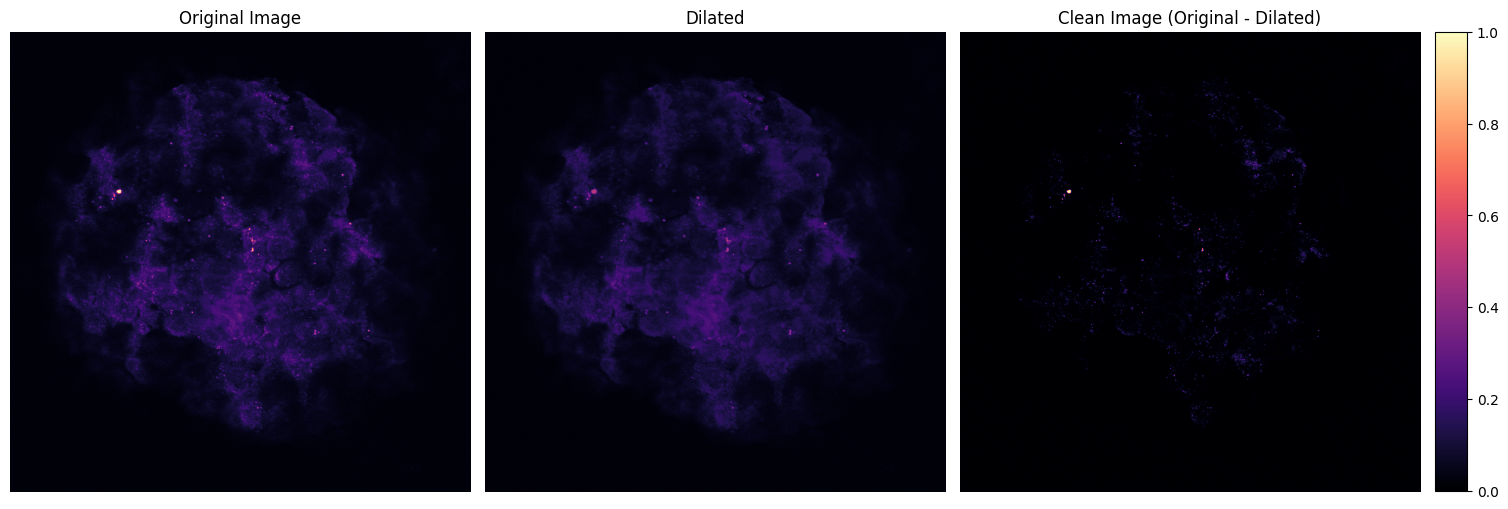
\includegraphics[width=\linewidth]{images/sph1_slice3/sox2_cleaning_improved.png}
    \caption{Cleaning of the SOX2 channel. From left to right: the original image, a dilated version of it (a blurred version or background noise), and the cleaned image as the difference between them. The original image corresponds to the SOX2 channel of \textsf{Sph1, slice3}. Note that the dilated image allows us to remove a large amount of non-informative pixels.  }
    \label{fig: sox2 before and after}
\end{figure}


\subsubsection*{The Nuclei Channel}
For this channel, we use the nuclei to individualize and identify the cells. Specifically, we performed instance segmentation on the nuclei, extracting geometrical features such as the area and the coordinates of the center of the segmented objects by the following the next steps: 

\begin{enumerate}
    \item Contrast Limited Adaptive Histogram Equalization (CLAHE): Used for local contrast enhancement (see \href{https://scikit-image.org/docs/stable/api/skimage.exposure.html#skimage.exposure.equalize_adapthist}{documentation}) makes the edge recognition easier for the segmentation algorithm.
    
    \item Morphological processing: To further improve the edge recognition, we performed a morphological opening (erosion followed by dilation), followed by an area closing (similar to a morphological closing, dilation followed by erosion, but using a deformable rather than a fixed footprint). The opening helps separate objects that may be in contact. The area closing removes small dark structures to avoid single nuclei being segmented as many objects due to dark spots within them (see \href{https://scikit-image.org/docs/stable/api/skimage.morphology.html#skimage.morphology.area_closing}{documentation}).
    
    \item Bilateral Denoising: An edge-preserving bilateral filter denoises the image, averaging pixels based on their spatial closeness and radiometric similarity. This filter works both to reduce the noise introduced by the morphology operations and by out-of-focus objects (see \href{https://scikit-image.org/docs/stable/api/skimage.restoration.html#skimage.restoration.denoise_bilateral}{ documentation}).
    
    \item Instance Segmentation: For identifying the nuclei, we used the \textsf{2D\_versatile\_fluo} model (see \href{https://github.com/stardist/stardist}{documentation}). This is a \textsf{Stardist} \cite{schmidt2018} convolutional neural network with a U-Net architecture, trained on fluorescence microscopy images similar to the ones of our experiment. 
    
    We chose this model instead of instance segmentation with bounding boxes because, in this way, we do not need a subsequent shape refinement. Furthermore, semantic (per-pixel) cell segmentation requires a subsequent pixel grouping that can result in segmentation errors such as falsely merging bordering cells. Since the images portray situations of very crowded cells,  such errors would be very likely to happen in our case. Star-convex polygons provide a much better shape representation that overcomes these difficulties.
\end{enumerate}

\begin{figure}[p]
    \centering
    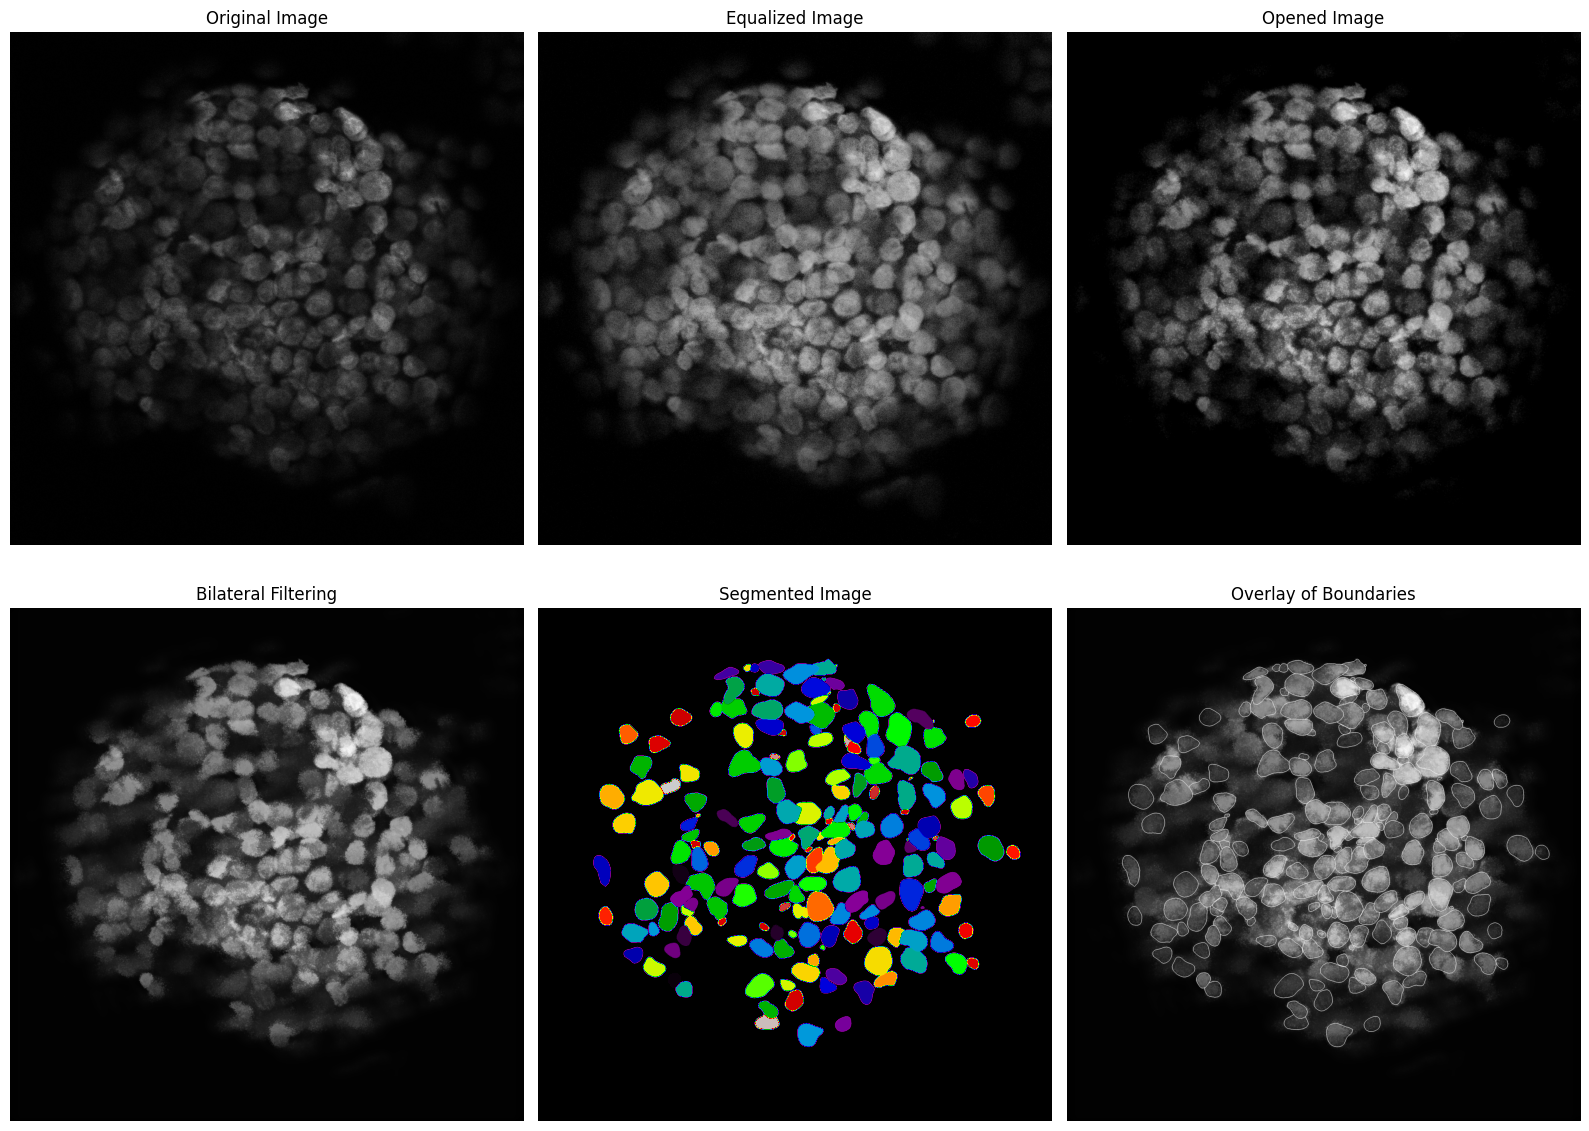
\includegraphics[width=\textwidth]{images/sph1_slice3/nuclei_processing_horizontal.png}
    \caption{Image processing of the nuclei fluorescence channel (DAPI). From left to right and top to bottom, the different steps in the processing of an image are followed. In the bottom right corner are shown the borders of the identified structures over the original image. The darker, unrecognized nuclei correspond to cells that are outside, in this case behind, the focal plane.}
    \label{fig: nuclei processing}
\end{figure}

The complete process on DAPI channel is depicted in Fig. \ref{fig: nuclei processing}. The original image is in the upper left corner. The lower right image is an enhanced representation highlighting the reconstructed cell boundaries.  


\subsubsection*{Tessellation for cell region identification}
Since the SOX2 marker is not necessarily bound to the nucleus of the cell, but rather to its cytoplasm, we need a way of assigning each point in space (i.e., each pixel) to a single cell to further associate the fluorescence of the marker with a given cell. To do this, we approximated the division of the space associated with each cell by a Voronoi tessellation. We used the centers of the segmented objects filtering out the ones corresponding to cells that do not belong to the spheroid when needed. The result is shown in Fig. \ref{fig: tessellation to clustered}A. It is worth mentioning that we used artificial points, uniformly distributed in a circumference enclosing the spheroid, to limit the area of the cells in its border.

\begin{figure}[h!]
   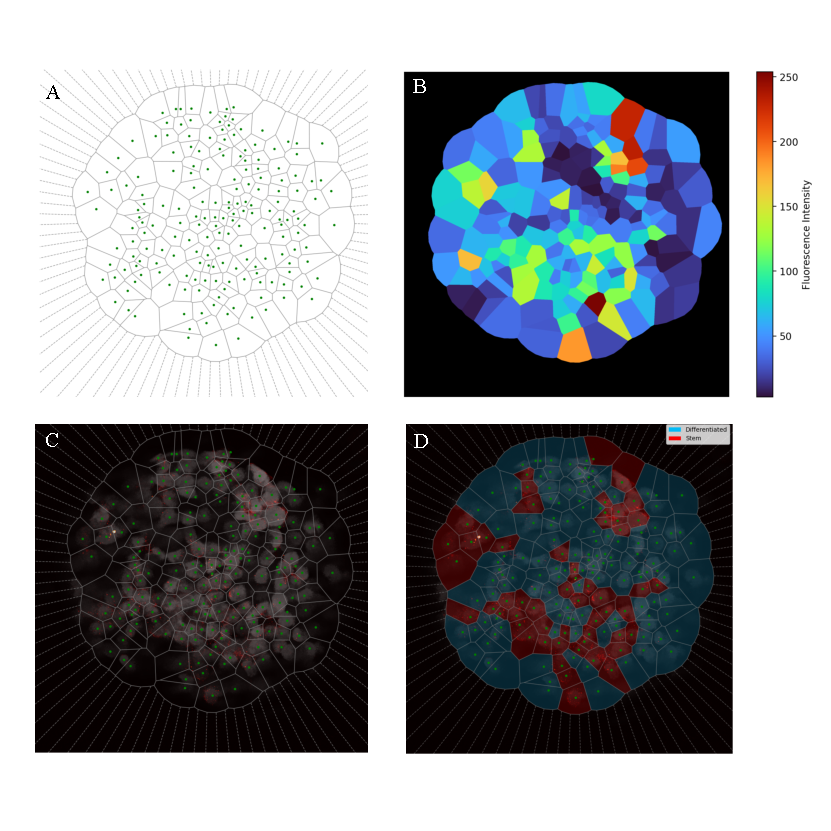
\includegraphics[width=\textwidth]{images/tessellation_to_csc_recognition.eps}
   \caption{From tessellation to CSC recognition. \textbf{A} Voronoi tessellation. The centroids of the cells, green dots, were used to estimate the cell area. \textbf{B} Regions colored according to SOX2 fluorescence intensity. For each region of the tessellation, the sum of its SOX2 fluorescence intensity is computed. \textbf{C} Tessellation overlaid with nuclei (gray scale) and SOX2 (red palette) channels. The boundaries between Voronoi regions are plotted with gray lines. \textbf{D} Tessellation regions are colored in red for Cancer Stem Cells and blue for Differentiated Cancer Cells, according to their SOX2 fluorescence content. If the fluorescence surpasses the threshold given by the GMM, the cell is considered a stem one.}
   \label{fig: tessellation to clustered}
\end{figure}

We thus associated to each cell, the sum of the fluorescence intensity of each pixel of the SOX2 channel contained inside its corresponding Voronoi region. The result of this association is shown in Fig. \ref{fig: tessellation to clustered} as a color scale depicting the amount of SOX2 in each Voronoi region. To better visualize the tessellation, we overlayed it on the nuclei fluorescence and the cleaned SOX2 channel in Fig. \ref{fig: tessellation to clustered}C.


\subsubsection*{Stemness threshold in SOX2 fluorescence intensity}

To identify the CSCs, is needed to define a threshold in the intensity of SOX2 fluorescence that divides non-stem from stem cells. We implemented a clustering algorithm to group the intensities of the cells and an ``elbow'' plot using k-means clustering. Its result, 2,  confirmed the suitability of our model with two cell phenotypes. Thus, we considered a fixed number of two groups were data points were assigned according to a Gaussian Mixture Model (GMM) fitted to the data. In short, we assumed that the points were generated by two normal distributions, fitting their means and standard deviations using the maximum likelihood criterion. Additional details can be found in the  \href{https://scikit-learn.org/stable/modules/generated/sklearn.mixture.GaussianMixture.html}{documentation}.

Since the fitting of the distributions is sensitive to extreme values, the outliers, below 5th and above 95th percentiles, were directly assigned to their corresponding category, differentiated for the lowest and stem for the highest values, and not were taken into account when fitting the GMM. An example of the histogram of SOX2 fluorescence intensities for \textsf{Sph1,slice 3} is shown in Fig. \ref{fig: filtered GMM histogram}. The threshold value $V=71.4$implies that from a total of $N=183$ cells present in the spheroid, $S_V=55$ are stem cells, a fraction of $f_V\simeq0.3$ of the total.
For every case, we checked that the random seed of the clustering algorithm had not modified the threshold significantly. Usually, there are a couple of values to which the threshold converges. Checking for robustness of the clustering means that these values are close to each other, regardless of the random state used and the clustering algorithm. If these values vary a lot or are not close to each other, the clustering becomes unreliable. For the case of our example, both GMM and K-means yield a threshold of 71.4, for a large number of random seeds.

A more intuitive way of visualizing this result is taking Fig. \ref{fig: tessellation to clustered}C and coloring each region according to its clustering. This is shown in Fig. \ref{fig: tessellation to clustered}D where, superimposed to the confocal image, the regions corresponding to stem cells are colored in red, and the regions corresponding to differentiated cells are colored in blue. 

The final result of the image processing is shown in Fig. \ref{fig: blue red}. There just the Voronoi regions are depicted as being colored according to their category. The image depicted in Fig. \ref{fig: blue red}C corresponds to the one in ig. \ref{fig: tessellation to clustered}D. 


\begin{figure}
    \centering
    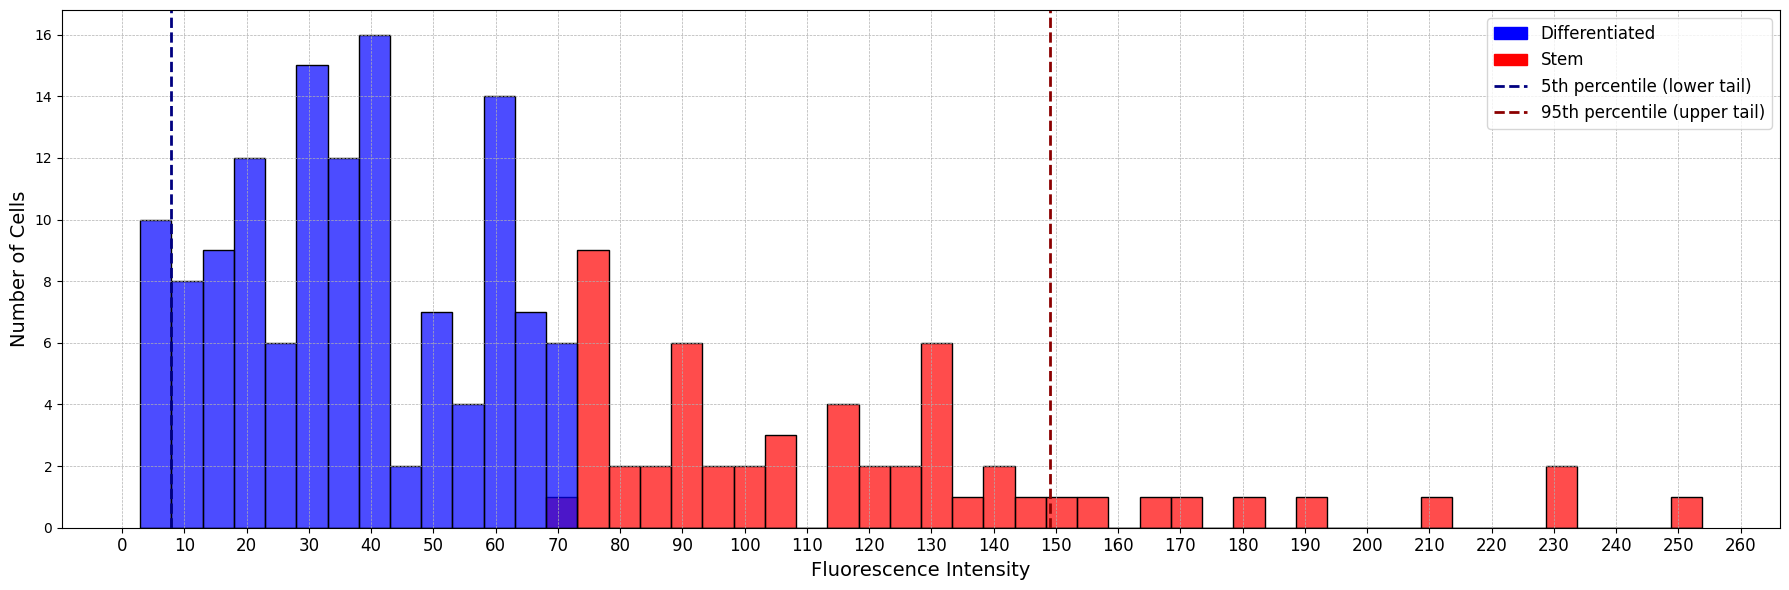
\includegraphics[width=1.0\textwidth]{images/sph1_slice3/histogram_GMM_clustering_cutting_tails_in_sph_NEW.png}
    \caption{Histogram of SOX2 fluorescence intensities, colored by the GMM clustering. Intensity values were clustered into differentiated and stem cells by fitting a GMM. Regions with intensities falling in the 5th  and  95th percentile were automatically considered as differentiated and stem respectively and were not taken into account when fitting the GMM.}
    \label{fig: filtered GMM histogram}
\end{figure}


\subsubsection*{CSC connectedness and path forming} \label{sss: csc connectedness}
The location of the CSCs seems to be far from random by visual inspection of Fig. \ref{fig: blue red}, since the paths that they form, break the homogeneity of their distribution. This intuition is confirmed by the graph of a \emph{Delaunay triangulation}, the dual lattice of the Voronoi tessellation. This is nothing else than the graph given by using the centroids of the Voronoi as nodes, and adding a link between two nodes if the corresponding cells in the Voronoi diagram are neighboring cells. For instance, in Fig. \ref{fig: Delaunay sph1 slice 3}{\bf A} we depict the network corresponding to {\textsf Sph1, slice3}, the red and blue dots correspond to CSCs and DCCs respectively. Also we studied the subgraph with just the CSCs shown in Fig. \ref{fig: Delaunay sph1 slice 3}{\bf B}. This graph is obtained by removing all the blue nodes and all the links connected to them. We used these isolated paths, to assess if two CSCs are neighboring by chance. Particularly, we look if the nodes of the network have preferential attachment for nodes of the same type. We calculated the \emph{homophily} of the graph, i.e. how much more likely are CSCs to be connected between them, than to DCCs. This was achieved by measuring, on the graphs, the following parameters:

\begin{figure}[h!]
        \centering
        \includegraphics[width=\textwidth]{images/network.eps}
    \caption{{\bf A} The reconstructed network for {\textsf Sph1, slice3} with its Cancer Stem Cells plotted as red dots while its Differentiated Cancer Cells plotted as blue dots. Neighbor cells are connected with gray links. {\bf B} The CSCs subgraph corresponding to the network in {\bf A} is obtained by deletion of the DCCs (blue) nodes. The number of stem/connected components is 5. {\bf C} The random graphs are constructed by randomly redistributing the red and blue dots on the same network. {\bf D} The  CSCs subgraph corresponding to the randomized network in {\bf C} has a different number of connected components, 13 in this case. In most random cases, this number is larger than in the experimental network. }
    \label{fig: Delaunay sph1 slice 3}
\end{figure}


\begin{itemize}
    \item \emph{Assortativity coefficient}: The measurement of preferential attachment that is used in network science. It is calculated as the Pearson correlation coefficient of the attribute indicating the type of cell, between pairs of linked nodes. The coefficient equals 1 for perfect assortativity (perfect preferential attachment), 0 for non-assortative networks (i.e., no preferential attachment), and -1 for perfectly disassortative networks (perfect heterophily).
    \item \emph{Homophily ratio}: Is the fraction of the edges of the graph that link nodes of the same kind. The calculation is direct, dividing the number of edges connecting cells of the same type by the total number of edges. 
    \item \emph{Number of stem-connected components}: At the subgraph formed by considering only the stem cells of the original graph and the links between them (stem subgraph), is the number of separated clusters. If stem cells form clusters, the number of connected components will be smaller than expected for a random distribution.
    \item \emph{Degree distribution of the stem subgraph}: In the stem subgraph is the average number of stem cells that are connected to each stem cell. For instance, if the mean degree is higher than expected for randomly distributed stem cells, it means that stem cells are more connected between them than what would be expected from the random case.
\end{itemize}
%
A \lstinline{NetworkX}'s\cite{SciPyProceedings_11} implementation was used for measuring all parameters, except for the homophily ratio. For more details consult the package's \href{https://networkx.org/documentation/stable/reference/algorithms/generated/networkx.algorithms.assortativity.attribute_assortativity_coefficient.html#networkx.algorithms.assortativity.attribute_assortativity_coefficient}{documentation}). 

We also look for the possibility that CSCs were placed at random positions. On the same networks obtained by Delaunay triangulation on the pictures, and leaving the connections untouched, we randomly redistributed the CSC in the graph. An example is shown in Fig. \ref{fig: Delaunay sph1 slice 3}{\bf C} where the red and blue dots are now randomly placed in other nodes, as seen when compared with the panel {\bf A}. In panel {\bf D} we depicted the subgraph corresponding to the randomized network of panel {\bf C}. Note that the number of connected components has increased from 5 in panel {\bf B} to 13 for this case, a situation that occurs for most randomized networks. We performed this relocation of the whole set of CSCs 10000 times and measured the mentioned parameters joined with their corresponding standard deviations. The results comparing both, experimental and randomized networks, are reported in Table \ref{tab: ensemble statistics}. We also performed statistical tests (z-test via \textsf{statsmodels} implementation \cite{seabold2010statsmodels}) to decide whether a given value could be obtained from the distribution of the sample, i.e. if the parameter is significantly different from the random case. In every case, we used a significance $\alpha_{t}=0.001$, but results are robust against even lower values of $\alpha_{t}$.


\bibliography{sample}


\section*{Acknowledgements }
The authors thank Dr. C. A. Condat for insightful discussions and comments. The confocal imaging was performed by .\todo{Luciano: poner CPA del MICROSCOPIO}

\section*{Funding}The theoretical work was supported by SECyT-UNC (Project 113/17) and CONICET (PIP 11220110100794), Argentina. Experiments were supported by \todo{FINANCIAMIEnTo LUCIANO}. 

\section*{Author contributions statement}

JF developed and implemented the image processing pipeline, LB conceived the general idea,  LV carried out the experiment. All authors analyzed the results and wrote the manuscript. 

\section*{Additional information}
\textbf{Competing interests}: The authors declare no competing interests.

\noindent \textbf{Accession codes}: All code and data are accessible through the GitHub repository: \href{https://github.com/JeroFotinos/experimental_image_analysis}{
\includegraphics[width=1em]{images/github-mark.pdf} \nolinkurl{experimental_image_analysis}}

%The corresponding author is responsible for submitting a \href{http://www.nature.com/srep/policies/index.html#competing}{competing interests statement} on behalf of all authors of the paper. This statement must be included in the submitted article file.

%\setcounter{figure}{0}   
\setcounter{page}{1}   
\setcounter{section}{0} 
\renewcommand\thefigure{S\arabic{figure}}



{\Huge Supplementary Material}

\section{Other examples}

Final reconstruction of CSC distribution for other samples shown in the text.

\begin{figure}[h!]
    \centering
    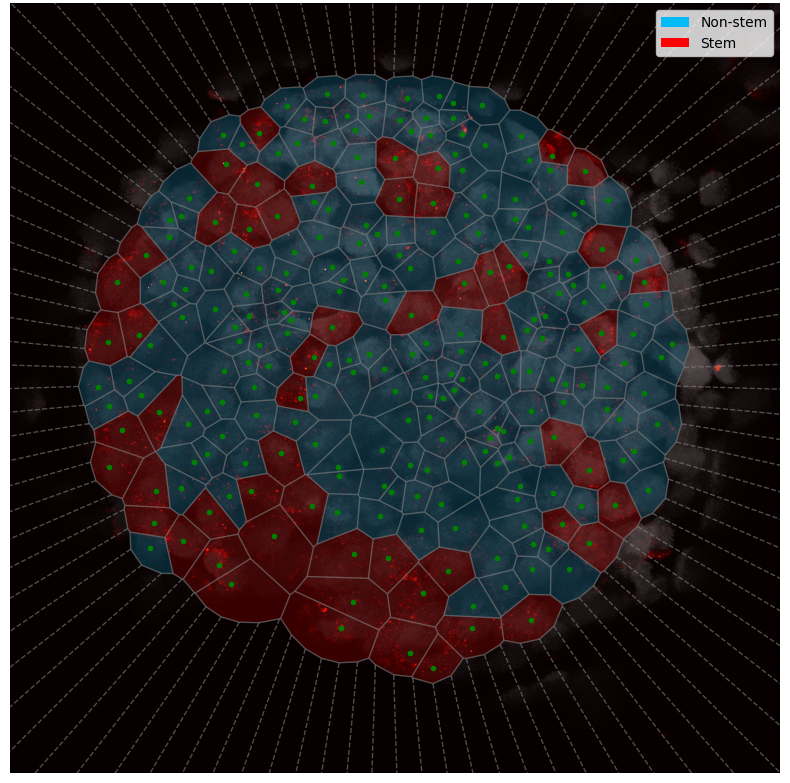
\includegraphics[width=0.8\textwidth]{images/sph1_slice4/nuclei_voronoi_in_sph_only_sox2_clustered_tails_cut_in_sph_with_artificial_boundary_cropped.png}
    \caption{\emph{Voronoi Tessellation overlaid with nuclei and SOX2 fluorescence, colored by stemness (slice 4, \lstinline{Sph1}).} The nuclei fluorescence is shown in a gray scale, whereas the SOX2 fluorescence is shown in a red palette. The centroids of the segmented nuclei are shown as green dots, and the boundaries between the Voronoi regions are plotted with gray lines. Regions have been colored in red (for stem) and blue (for non-stem ones) according to their SOX2 fluorescence content. This layer of cells is below the one seen in Fig. \ref{fig: nuclei voronoi sox2 clustered}. Note how cells that do not belong to the spheroid don't get a region in the tessellation.}
    \label{fig: nuclei voronoi sox2 clustered slice 4}
\end{figure}


\begin{figure}[h!]
    \centering
    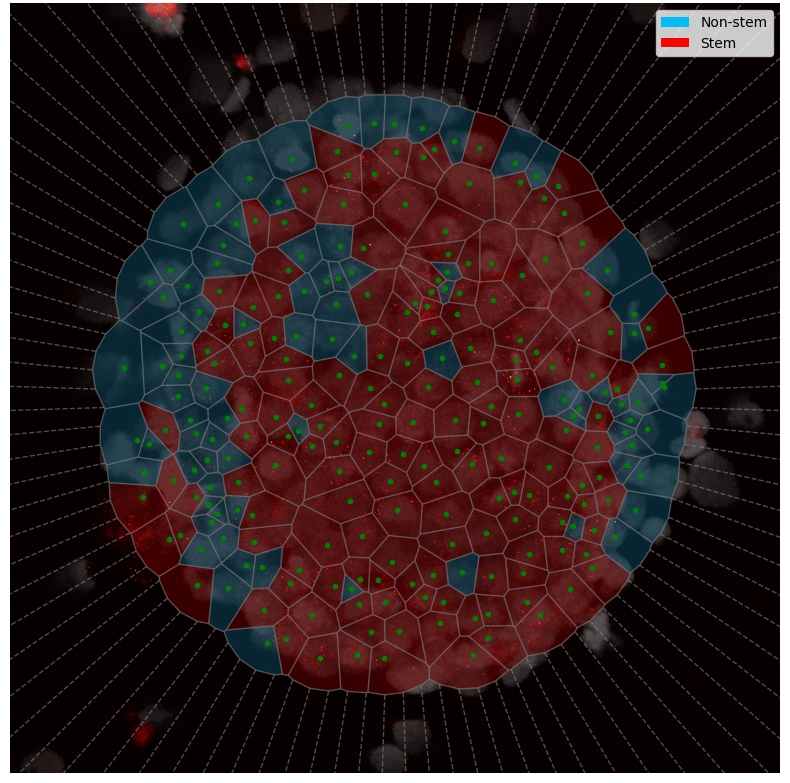
\includegraphics[width=0.8\textwidth]{images/sph3_slice3/nuclei_voronoi_in_sph_only_sox2_clustered_tails_cut_in_sph_with_artificial_boundary_cropped.png}
    \caption{\emph{Voronoi Tessellation overlaid with nuclei and SOX2 fluorescence, colored by stemness (slice 3, \lstinline{Sph3}).} The nuclei fluorescence is shown in a gray scale, whereas the SOX2 fluorescence is shown in a red palette. The centroids of the segmented nuclei are shown as green dots, and the boundaries between the Voronoi regions are plotted with gray lines. Regions have been colored in red (for stem) and blue (for non-stem ones) according to their SOX2 fluorescence content. If the fluorescence surpasses the threshold given by the GMM, the cell is considered a stem one. Regions further away than a certain threshold from the center of the spheroid were excluded from the clustering. Those regions were taken into account for associating the SOX2 to each cell, but their Voronoi cells are not drawn.}
    \label{fig: nuclei voronoi sox2 clustered sph3 slice 3}
\end{figure}




% \section{Delauny triangulation}

% \begin{figure}[h!]
%     \centering
%     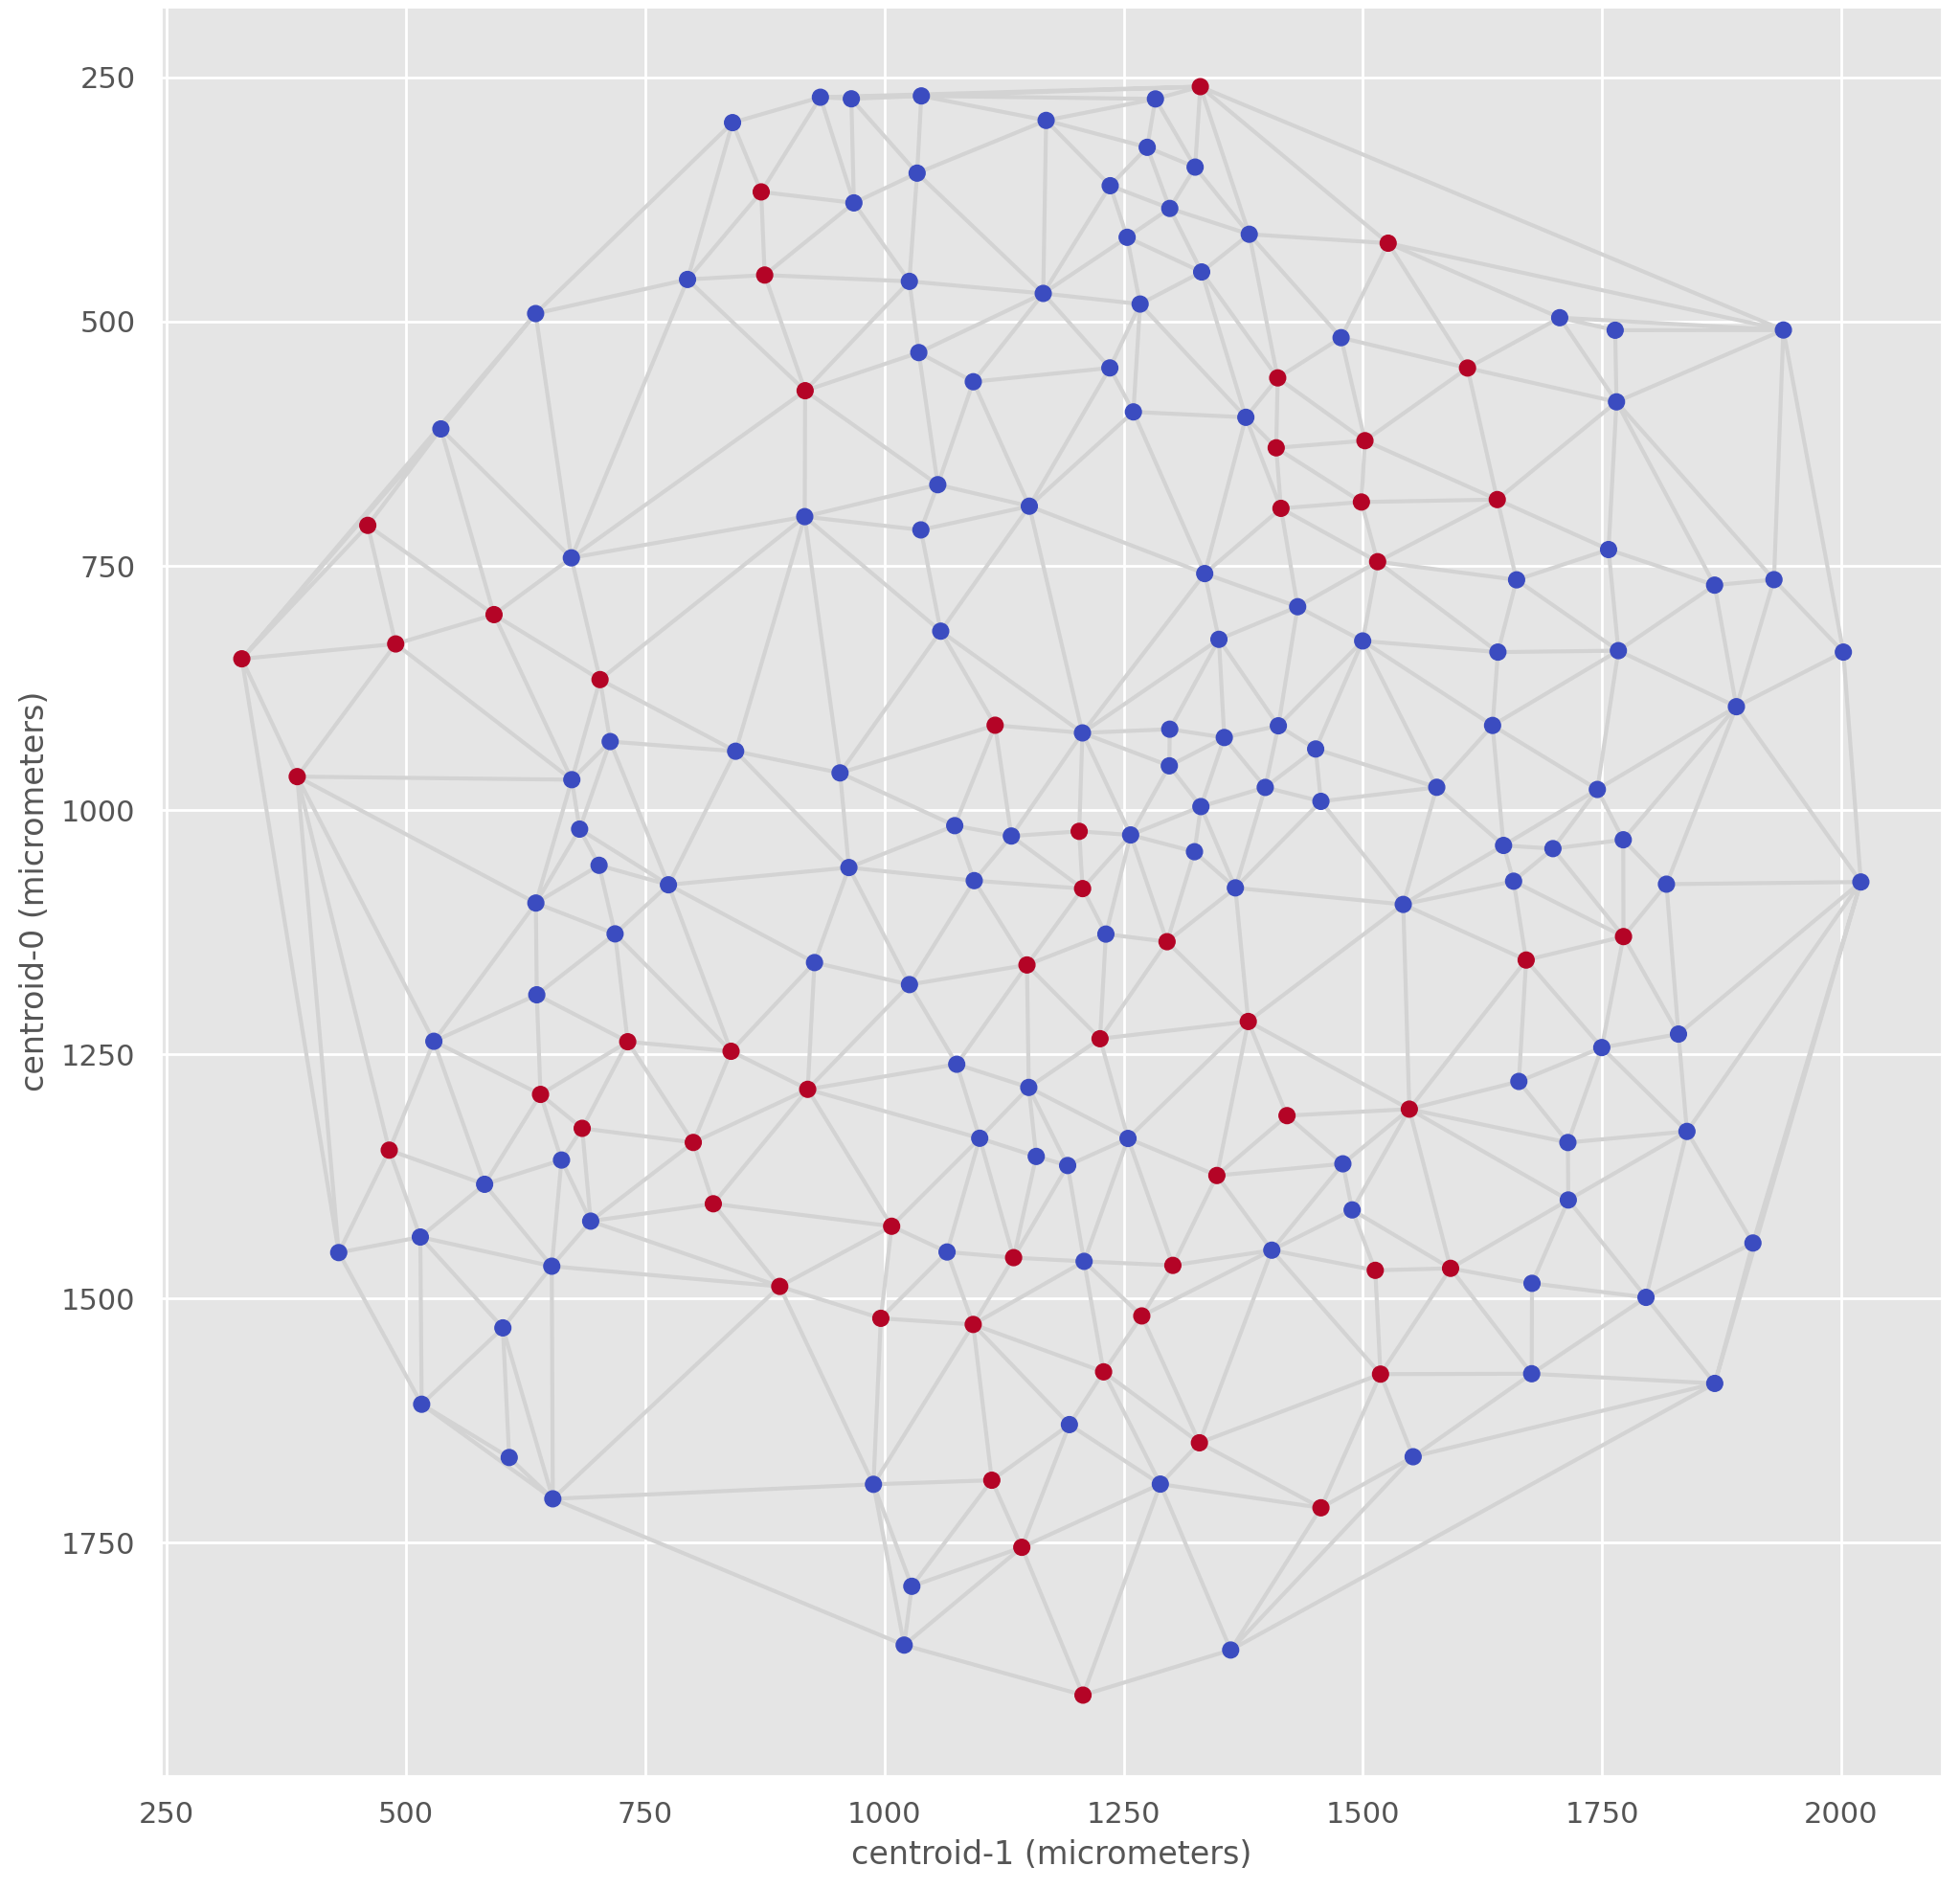
\includegraphics[width=0.9\textwidth]{images/sph1_slice3/delaunay_cropped.png}
%     \caption{\emph{Delaunay triangulation (slice 3, \lstinline{Sph1}).} The network shows Voronoi regions as nodes, and adjacency between regions as edges. Regions corresponding to stem cells are plotted as red dots, while differentiated cells are plotted as blue dots. The axis represent spatial coordinates in the focal plane, measured in micrometers.}
%     \label{fig: Delaunay sph1 slice 3}
% \end{figure}


\end{document}